% 3.1.Cmake.tex
%	Last update: 2021/05/17 F.Kanehori
%\newpage
\subsection{CMake}
\label{subsec:CMake}
\parindent=0pt

CMakeにはConfigureとGenerateの2段階があります。

\medskip
コマンドプロンプトの場合は、1回のコマンドで両方を実行できます。
\Vskip{-.5\baselineskip}

\CmndLine{%
	> chdir .../Springhead\\
	> mkdir build\\
	> cmake -B build [\it{generator}]
}{chap-3-1-cmake-cui.eps}{cmake cui}

\medskip
\it{generatorの}詳細は、コマンドプロンプトで\tt{cmake --help}とすると確認できます。

\it{generator}を省略した場合のデフォルトは、unixではMakefileが選択されます。
またWindowsの場合には、
インストールされているVisual Studioの最新バージョンがが選択されるようです。
ただし、マシンアーキテクチャは自動的には判定されません。
64ビットマシンの場合には \tt{-A x64}を指定してください。
これを忘れるとVisual Studioのプラットフォームが\tt{x64}となりません。

\begin{narrow}[s]
	\Vskip{-.2\baselineskip}\thinrule{\linewidth}\\
	\hspace{5pt}\it{generator}の例\\
	\begin{tabular}{@{\hspace{15pt}}l@{\hspace{10pt}}l}
	    Windows:	& \tt{-G "Visual Studio 15 2017" -A x64} \\
	    unix:	& \tt{-G "Unix Makefiles"} \\
	\end{tabular}\\
	\Vskip{-.2\baselineskip}\thinrule{\linewidth}\\
\end{narrow}

\bigskip
cmake--guiを利用する場合は、
まず、次の画面でConfigureボタンを押します。
\newpage
\begin{narrow}[15pt]
	\begin{figure}[h]
	\begin{center}
	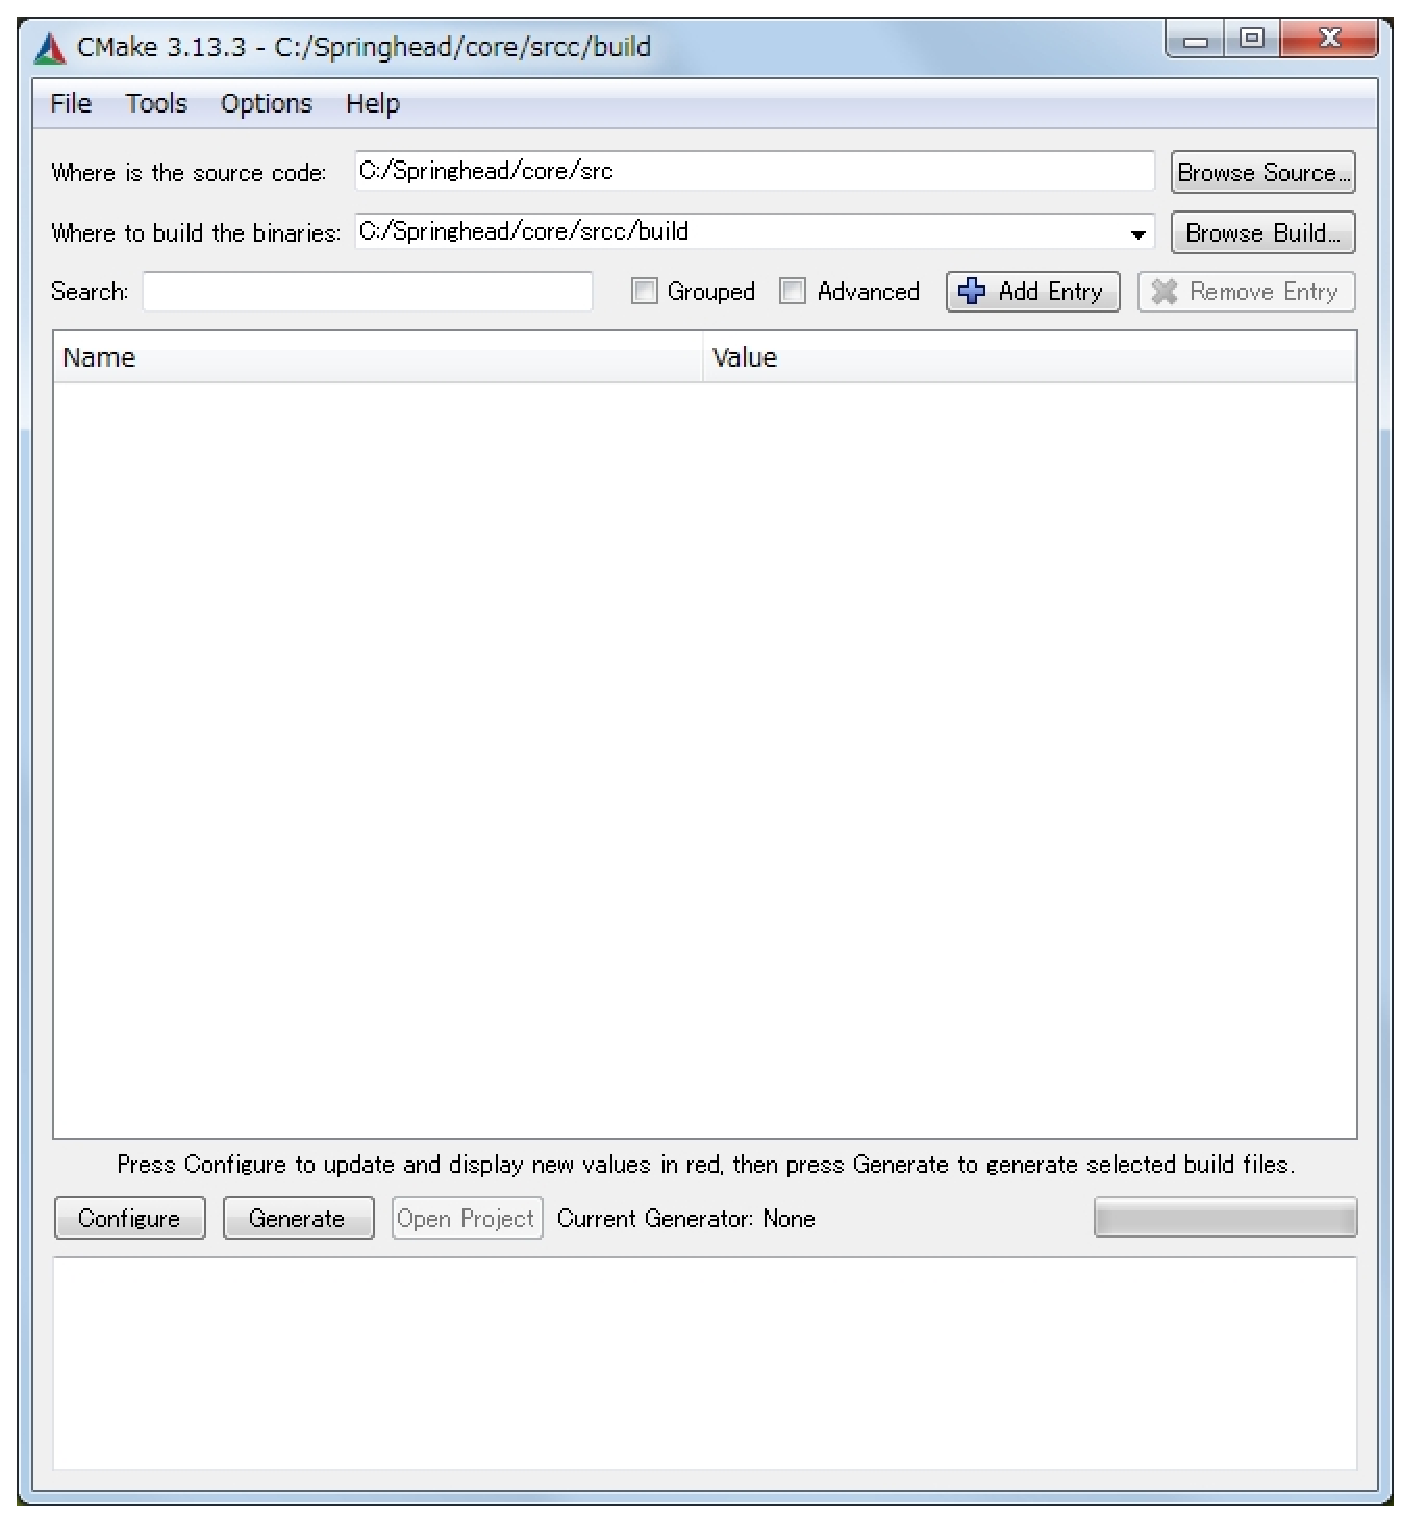
\includegraphics[width=0.7\textwidth]{fig/CmakeConfigure1.eps}
	\end{center}
	\caption{\cmake\ configure}
	\label{fig:CmakeConfigure}
	\end{figure}
\end{narrow}

\DQuote{\BldDir}ディレクトリがなければ作成するかどうかを尋ねられ、
\begin{narrow}[15pt]
	\begin{figure}[h]
	\begin{center}
	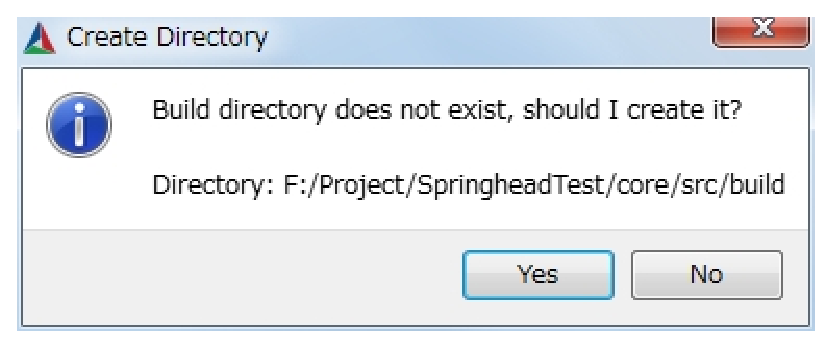
\includegraphics[width=0.5\textwidth]{fig/CmakeConfigure2.eps}
	\end{center}
	\caption{\cmake\ configure}
	\label{fig:CreateWorkSpace}
	\end{figure}
\end{narrow}

次にgenerator指定画面となります。
\begin{narrow}[15pt]
	\begin{figure}[h]
	\begin{center}
	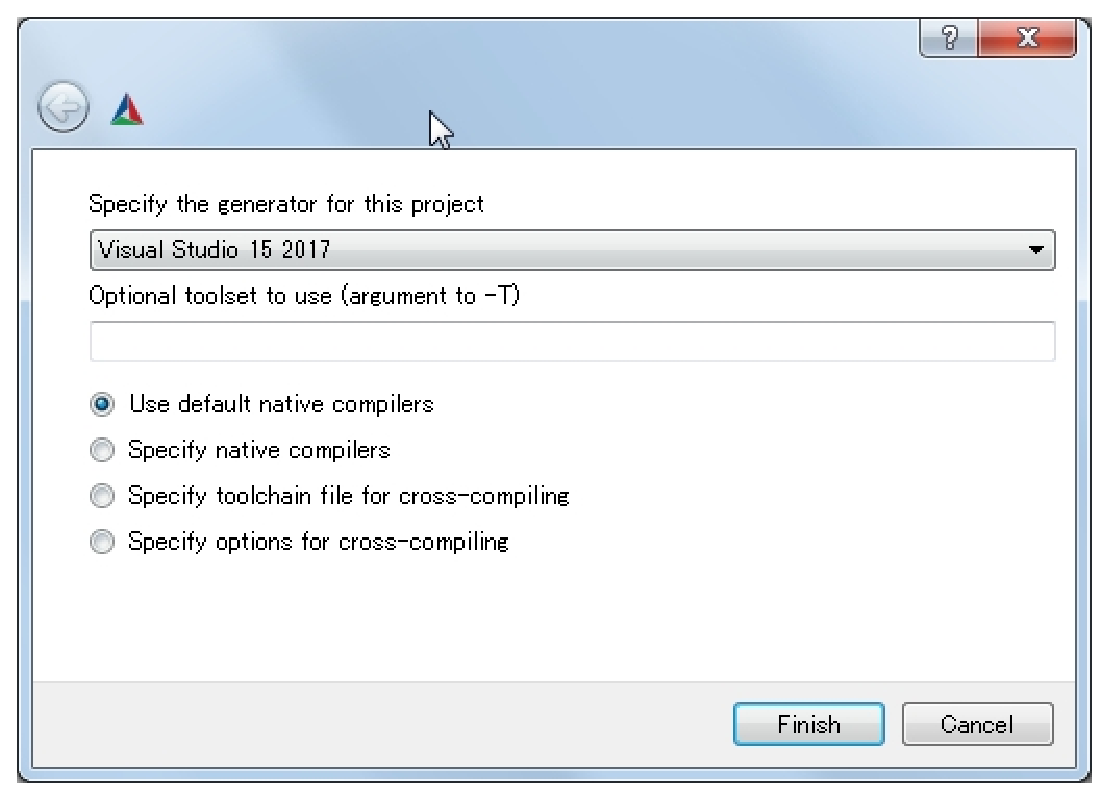
\includegraphics[width=0.6\textwidth]{fig/CmakeConfigure3.eps}
	\end{center}
	\caption{\cmake\ configure}
	\label{fig:CmakeGeneration}
	\end{figure}
\end{narrow}

最後に図\ref{fig:CmakeConfigure} のGenerateボタンを押します。

\medskip
以上で、\DQuote{\BldDir}以下にMakefile (unixの場合)
またはsolution/project file (Windowsの場合)
が生成されたはずです。

\bigskip
% end: 3.1.Cmake.tex
